\documentclass{article}

%\usepackage{lmodern}
\usepackage{inputenc}
%\renewcommand*\familydefault{\sfdefault}

\usepackage{amsmath}
\usepackage{tikz}
\usetikzlibrary{matrix}

\usepackage{amsmath}
\usepackage{algorithm}
\usepackage[noend]{algpseudocode}
\usepackage{minted}
\usemintedstyle{monokai}
\usepackage{xcolor}
\usepackage{enumitem}
\setenumerate[0]{label=(\alph*)}


\makeatletter
\def\BState{\State\hskip-\ALG@thistlm}
\makeatother



\usepackage{array,mathtools}
\newcommand*{\carry}[1][1]{\overset{#1}}
\newcolumntype{B}[1]{r*{#1}{@{\,}r}}

% expandable loop (used to avoid scope problems in tabular cells with the
% standard \loop)
\def\boucle #1\repeat {#1\b@@cle {#1}\repeat \repeat }
\def\b@@cle #1{\repeat #1\b@@cle {#1}}

\makeatletter
\newcount\@nn
\newcount\@mm
\newcount\@base
\newcount\@baseminusone

% please do not use this at home
% #1 must be a counter name, not something expanding to a number.
\def\@arabalpha #1{\ifcase #10\or1\or2\or3\or4\or5\or6\or7\or8\or9\or 
A\or B\or C\or D\or E\or F\or G\or H\or I\or J\or K\or L\or M\or N\or O\or
P\or Q\or R\or S\or T\or U\or V\or W\or X\or Y\or Z\fi}

\newcommand{\baseexpansion}[2][2]{% no negative numbers please!
\def\@digits{}%
\@base#1\relax \@baseminusone\@base\advance\@baseminusone-1
\@nn #2\relax  % this is the number to be written in base #1
%
\ifnum\@baseminusone<36
\def\onerow{#1\kern.1em\hbox{\vrule
   \vtop {\hbox{\ \the\@nn}\kern.3ex\hrule height.1ex }} &%
   \global\@mm\@nn \global\divide\@mm\@base 
   \multiply\@mm\@base \advance\@nn-\@mm 
   \the\@nn \xdef\@digits{\@arabalpha\@nn\@digits}}%
\else
\def\onerow{#1\kern.1em\hbox{\vrule
   \vtop {\hbox{\ \the\@nn}\kern.3ex\hrule height.1ex }} &%
   \global\@mm\@nn \global\divide\@mm\@base 
   \multiply\@mm\@base \advance\@nn-\@mm 
   \the\@nn \xdef\@digits{\the\@nn.\@digits}}%
\fi
%
\leavevmode\oalign{$#2_{10}:$\hfil\cr
      $\left.
      \begin{tabular}{r|l}
         \boucle \onerow \\ \ifnum\@nn>\@baseminusone\global\@nn\@mm \repeat
      \end{tabular}\right\rbrace=
      \mathtt{\@digits}_{#1}$}}     % \hfil removed from the macro

\makeatother


\title{Tutorato Architettura degli Elaboratori Modulo 1 \\ Lezione 1}
\author{Francesco Pelosin}
\date{16 Ottobre 2019}

\begin{document}

\maketitle

\section{Conversione di base}
\subsection{Base $b$ $\rightarrow$ Base 10}

Dato un numero di $n$ cifre espresso in una qualsiasi base $b$:

$$d_{n-1}, d_{n-2}, \dots, d_{1}, d_{0}$$

\noindent Possiamo esprimerlo in base $10$ nel seguente modo:

$$d_{n-1}\cdot b^{n-1} + d_{n-2}\cdot b^{n-2} + \dots + d_{1} \cdot b^{1} + d_{0}\cdot b^{0}$$

\subsubsection*{Esercizi}

Tradurre i seguenti numeri in base $10$:
\begin{enumerate}
    \item $11310_{5}$
    \item $147_{12}$
    \item $3A7_{16}$
    \item $1703_{8}$
\end{enumerate}

\subsubsection*{Soluzioni}
\begin{enumerate}
    \item $11310_{5}=1\cdot 5^{4}+1\cdot 5^{3}+3\cdot 5^{2}+1\cdot5^{1}+0\cdot 5^{0}=625+125+75+5=830_{10}$
    \item $147_{12}=1\cdot 12^{2}+4\cdot 12^{1}+7\cdot 12^{0}=144+48+7=199_{10}$
    \item $3A7_{16}=3\cdot 16^{2}+10\cdot 16^{1}+7\cdot 16^{0}=768+160+7=935_{10}$
    \item $1703_{8}=1\cdot 8^{3}+7\cdot 8^{2}+0\cdot 8^{1}+3\cdot 8^{0}=512+448+3=963_{10}$
\end{enumerate}

\subsection{Base 10 $\rightarrow$ Base $b$}

Dato un numero $n$ espresso in base $10$ \`e possibile tradurlo in base $b$ applicando il seguente algoritmo.

\begin{algorithm}
\caption{Base$_{10}$ $\rightarrow$ Base$_{b}$ (Conversione Inversa) }
\begin{algorithmic}[1]
\Procedure{ConversioneInversa}{$n, b$}
\State $Q \gets n$
\State $i \gets 0$
\While{$Q>0$}
\State $d_{i}=Q \mod b$ \Comment{Resto della divisione per $b$}
\State print $d_{i}$
\State $Q = Q / b$  \Comment{Divisione intera}
\State $i=i+1$
\EndWhile
\EndProcedure
\end{algorithmic}
\end{algorithm}


\subsubsection*{Esercizi}
Tradurre i seguenti numeri nella base richiesta:
\begin{enumerate}
    \item $310_{10} \rightarrow$ in Base 6
    \item $321_{10} \rightarrow$ in Base 2
    \item $519_{10} \rightarrow$ in Base 5
    \item $1006_{10} \rightarrow$ in Base 9
\end{enumerate}

\subsubsection*{Soluzioni}

\textbf{N.B.:} la notazione es.: $6|310$ significa ``310/6''.

\lineskip12pt
\begin{enumerate}
  \item \baseexpansion[6]{310}\hfil
  \item \baseexpansion{321}\hfil
  \item \baseexpansion[5]{519}\hfil
  \item \baseexpansion[9]{1006}\hfil
\end{enumerate}

\subsubsection*{Esercizi}
Convertire i seguenti numeri da Base 10 a Base 2:
\begin{enumerate}
    \item $136_{10}$
    \item $192_{10}$
    \item $255_{10}$
    \item $35_{10}$
    \item $63_{10}$
\end{enumerate}
Convertire i seguenti numeri da Base 2 a Base 10:
\begin{enumerate}
    \item $100011_{2}$
    \item $101100_{2}$
    \item $111111_{2}$
    \item $10001000_{2}$
    \item $11000000_{2}$
    \item $11111111_{2}$
\end{enumerate}

\subsubsection*{Soluzioni}
\textbf{N.B.:} la notazione es.: $2|136$ significa ``136/2''.
\lineskip12pt
\begin{enumerate}
  \item \baseexpansion{136}\hfil
  \item \baseexpansion{192}\hfil
  \item \baseexpansion{255}\hfil
  \item \baseexpansion{35}\hfil
  \item \baseexpansion{63}\hfil
\end{enumerate}

\begin{enumerate}
    \item $100011_{2}=1\cdot 2^{5}+0\cdot 2^{4}+0\cdot 2^{3}+0\cdot 2^{2}+1\cdot 2^{1}+1\cdot 2^{0}=32+2+1=35_{10}$
    \item $101100_{2}=1\cdot 2^{5}+0\cdot 2^{4}+1\cdot 2^{3}+1\cdot 2^{2}+0\cdot 2^{1}+0\cdot 2^{0}=32+8+4=44_{10}$
    \item $111111_{2}=1\cdot 2^{5}+1\cdot 2^{4}+1\cdot 2^{3}+1\cdot 2^{2}+1\cdot 2^{1}+1\cdot 2^{0}=32+16+8+4+2+1=63_{10}$
    \item $10001000_{2}=1\cdot 2^{7}+0\cdot 2^{6}+0\cdot 2^{5}+0\cdot 2^{4}+1\cdot 2^{3}+0\cdot 2^{2}+0\cdot 2^{1}+0\cdot 2^{0}=128+8=136_{10}$
    \item $11000000_{2}=1\cdot 2^{7}+1\cdot 2^{6}+0\cdot 2^{5}+0\cdot 2^{4}+0\cdot 2^{3}+0\cdot 2^{2}+0\cdot 2^{1}+0\cdot 2^{0}=128+64=192_{10}$
    \item $11111111_{2}=1\cdot 2^{7}+1\cdot 2^{6}+1\cdot 2^{5}+1\cdot 2^{4}+1\cdot 2^{3}+1\cdot 2^{2}+1\cdot 2^{1}+1\cdot 2^{0}=128+64+32+16+8+4+2+1=255_{10}$
\end{enumerate}

\subsection{Base 2 $\rightarrow$ Base 8 (o Base 16)}

\textbf{Ricorda:} Dato un sistema numerico in base $b$ e date $n$ cifre diverse, possiamo rappresentare $b^{n}$ numeri diversi.\\

\noindent Considerando il sistema numerico binario a $3$ cifre, possiamo rappresentare $2^{3}=8$ numeri diversi, tuttavia gli stessi sono rappresentabili attraverso una sola cifra nel sistema numerico ottale (Base 8). Lo stesso principio si estende a $4$ cifre in relazione alla base esadecimale (Base 16). Infatti, considerando il sistema numerico binario a $4$ cifre, possiamo rappresentare $2^{4}=16$ numeri diversi, gli stessi possono essere codificati con un unico simbolo in base esadecimale. \\

\noindent Di conseguenza dovendo trasformare un numero binario in un numero ottale (o esadecimale) possiamo semplicemente raggruppare i bit a gruppi di 3 (o 4) e scrivere il loro corrispettivo valore in Base 8 (o Base 16). Possiamo sfruttare questa propriet\`a per velocizzare la conversione. Volendo ora applicare il procedimento inverso, ossia passare da Base 8 (o Base 16) a Base 2, baster\`a trasformare ogni cifra del numero nel corrispettivo binario ed esprimerla su 3 (o 4) bit.

\subsubsection*{Esercizi}
Tradurre i seguenti numeri da ottale a binario:
\begin{enumerate}
    \item $1242_{8}$
    \item $364_{8}$
    \item $673_{8}$
    \item $371_{8}$
    \item $536_{8}$
    \item $7325_{8}$
\end{enumerate}
Tradurre i seguenti numeri da esadecimale a binario:
\begin{enumerate}
    \item E3D$_{16}$
    \item AB4$_{16}$
    \item F8C$_{16}$
    \item 962$_{16}$
    \item 34A$_{16}$
    \item BF4$_{16}$
\end{enumerate}
Tradurre i seguenti numeri da binario a ottale:
\begin{enumerate}
    \item 100011111\textsubscript{2} $\rightarrow$ Base 8
    \item 011110011\textsubscript{2} $\rightarrow$ Base 8
    \item 101010111\textsubscript{2} $\rightarrow$ Base 8
\end{enumerate}
Tradurre i seguenti numeri da binario a esadecimale:
\begin{enumerate}
    \item 111101011010\textsubscript{2} $\rightarrow$ Base 16
    \item 101111100100\textsubscript{2} $\rightarrow$ Base 16
    \item 011010010010\textsubscript{2} $\rightarrow$ Base 16
\end{enumerate}

\subsubsection*{Soluzioni}
Soluzioni da ottale a binario:
\begin{enumerate}

    \item 1242\textsubscript{8}$=$(1\textsubscript{\underline{001}}2\textsubscript{\underline{010}}4\textsubscript{\underline{100}}2\textsubscript{\underline{010}})$=$001 010 100 010\textsubscript{2}
    \item 364\textsubscript{8}$=$(3\textsubscript{\underline{011}}6\textsubscript{\underline{110}}4\textsubscript{\underline{100}})$=$011 110 100\textsubscript{2}
    \item 673\textsubscript{8}$=$(6\textsubscript{\underline{110}}7\textsubscript{\underline{111}}3\textsubscript{\underline{011}})$=$110 111 011\textsubscript{2}
    \item 371\textsubscript{8}$=$(3\textsubscript{\underline{011}}7\textsubscript{\underline{111}}1\textsubscript{\underline{001}})$=$011 111 001\textsubscript{2}
    \item 536\textsubscript{8}$=$(5\textsubscript{\underline{101}}3\textsubscript{\underline{011}}6\textsubscript{\underline{110}})$=$101 011 110\textsubscript{2}
    \item 7325\textsubscript{8}$=$(7\textsubscript{\underline{111}}3\textsubscript{\underline{011}}2\textsubscript{\underline{010}}5\textsubscript{\underline{101}})$=$111 011 010 101\textsubscript{2}
\end{enumerate}
Soluzioni da esadecimale a binario:
\begin{enumerate}
    \item E3D\textsubscript{16}$=$(E\textsubscript{\underline{1110}}3\textsubscript{\underline{0011}}D\textsubscript{\underline{1101}})$=$1110 0011 1101\textsubscript{2}
    \item AB4\textsubscript{16}$=$(A\textsubscript{\underline{1010}}B\textsubscript{\underline{1011}}4\textsubscript{\underline{0100}})$=$1010 1011 0100\textsubscript{2}
    \item F8C\textsubscript{16}$=$(F\textsubscript{\underline{1111}}8\textsubscript{\underline{1000}}C\textsubscript{\underline{1100}})$=$1111 1000 1100\textsubscript{2}
    \item 962\textsubscript{16}$=$(9\textsubscript{\underline{1001}}6\textsubscript{\underline{0110}}2\textsubscript{\underline{0010}})$=$1001 0110 0010\textsubscript{2}
    \item 34A\textsubscript{16}$=$(3\textsubscript{\underline{0011}}4\textsubscript{\underline{0100}}A\textsubscript{\underline{1010}})$=$0011 0100 1010\textsubscript{2}
    \item BF4\textsubscript{16}$=$(B\textsubscript{\underline{1011}}F\textsubscript{\underline{1111}}4\textsubscript{\underline{0100}})$=$1011 1111 0100\textsubscript{2}
\end{enumerate}
Soluzioni da binario a ottale:
\begin{enumerate}

    \item 100011111\textsubscript{2}$=$(100\textsubscript{\underline{4}}011\textsubscript{\underline{3}}111\textsubscript{\underline{7}})$=$4 3 7\textsubscript{8}
    \item 011110011\textsubscript{2}$=$(011\textsubscript{\underline{3}}110\textsubscript{\underline{6}}011\textsubscript{\underline{3}})$=$3 6 3\textsubscript{8}
    \item 101010111\textsubscript{2}$=$(101\textsubscript{\underline{5}}010\textsubscript{\underline{2}}111\textsubscript{\underline{7}})$=$5 2 7\textsubscript{8}
\end{enumerate}
Soluzioni da binario a esadecimale:
\begin{enumerate}

    \item 111101011010\textsubscript{2}$=$(1111\textsubscript{\underline{15=F}}0101\textsubscript{\underline{5}}1010\textsubscript{\underline{10=A}})$=$F 5 A\textsubscript{16}
    \item 101111100100\textsubscript{2}$=$(1011\textsubscript{\underline{11=B}}1110\textsubscript{\underline{14=E}}0100\textsubscript{\underline{4}})$=$B E 4\textsubscript{16}
    \item 011010010010\textsubscript{2}$=$(0110\textsubscript{\underline{6}}1001\textsubscript{\underline{9}}0010\textsubscript{\underline{2}})$=$6 9 2\textsubscript{16}
\end{enumerate}

\section{Somma tra numeri binari senza segno}

Le operazioni di somma sono eseguite in colonna bit a bit applicando un procedimento analogo a quello per le somme in decimale su carta.
La somma di numeri binari senza segno produce overflow se e soltanto se il risultato \`e troppo grande per essere rappresentato nel numero finito di bit messo a disposizione (ossia se il riporto pi\`u significativo \`e a 1).

\subsubsection*{Esercizi}
Eseguire le seguenti somme tra numeri binari senza segno su 8 bit. Discutere l'overflow motivando la risposta. Se i numeri sono espressi in decimale eseguire prima la traduzione in binario.

\begin{enumerate}
    \item 11010110\textsubscript{2}+00111010\textsubscript{2}
    \item 11011100\textsubscript{2}+00011111\textsubscript{2}
    \item 00111111\textsubscript{2}+11000000\textsubscript{2}
    \item 136\textsubscript{10}+192\textsubscript{10}
    \item 136\textsubscript{10}+35\textsubscript{10}
    \item 63\textsubscript{10}+44\textsubscript{10}
\end{enumerate}


\subsubsection*{Soluzioni}
\textbf{N. B.:} Ogni somma bit a bit scrive sopra di essa il riporto generato.
\begin{enumerate}
\item 11010110\textsubscript{2}+00111010\textsubscript{2}=00010000\textsubscript{2} $\Rightarrow$ ultimo riporto uguale a 1 $\Rightarrow$ overflow

\begin{center}
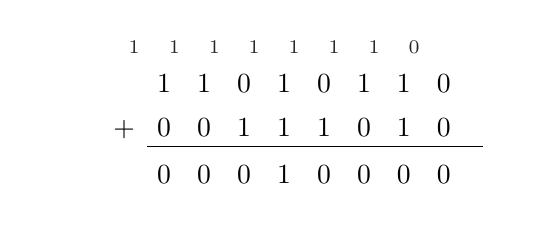
\begin{tikzpicture}[
    row 1/.style={font=\textsl,font=\scriptsize,black!85, anchor=west,
        inner sep=1.5pt},
    every node/.style={column sep=.5mm,row sep=1mm}]
    \matrix (m) [matrix of math nodes,
        nodes in empty cells,
        %nodes=draw
    ] 
    {
        &  &  & 1 & 1 & 1  & 1 & 1 & 1 & 1 & 0 &    &  &                   \\
        &  &  &   & 1 & 1  & 0 & 1 & 0 & 1 & 1 & 0  &  &[10mm]      \\
        &  &  & + & 0 & 0  & 1 & 1 & 1 & 0 & 1 & 0  &  &            \\ 
        &  &  &   & 0 & 0  & 0 & 1 & 0 & 0 & 0 & 0  &  &            \\                                                  
    };

    \draw[-,color=black,semithick] (m-3-5.south west) -- (m-3-13.south east);

\end{tikzpicture}
\end{center}


\item 11011100\textsubscript{2}+00011111\textsubscript{2}=11111011\textsubscript{2} $\Rightarrow$ ultimo riporto uguale a 0 $\Rightarrow$ no overflow

\begin{center}
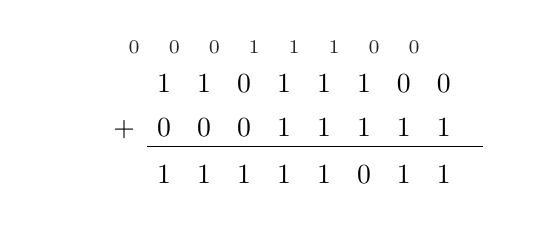
\begin{tikzpicture}[
    row 1/.style={font=\textsl,font=\scriptsize,black!85, anchor=west,
        inner sep=1.5pt},
    every node/.style={column sep=.5mm,row sep=1mm}]
    \matrix (m) [matrix of math nodes,
        nodes in empty cells,
        %nodes=draw
    ] 
    {
        &  &  & 0 & 0 & 0  & 1 & 1 & 1 & 0 & 0 &    &  &                   \\
        &  &  &   & 1 & 1  & 0 & 1 & 1 & 1 & 0 & 0  &  &[10mm]      \\
        &  &  & + & 0 & 0  & 0 & 1 & 1 & 1 & 1 & 1  &  &            \\ 
        &  &  &   & 1 & 1  & 1 & 1 & 1 & 0 & 1 & 1  &  &            \\                                                  
    };

    \draw[-,color=black,semithick] (m-3-5.south west) -- (m-3-13.south east);

\end{tikzpicture}
\end{center}
\item 00111111\textsubscript{2}+11000000\textsubscript{2}=11001000\textsubscript{2} $\Rightarrow$ ultimo riporto uguale a 0 $\Rightarrow$ no overflow

\begin{center}
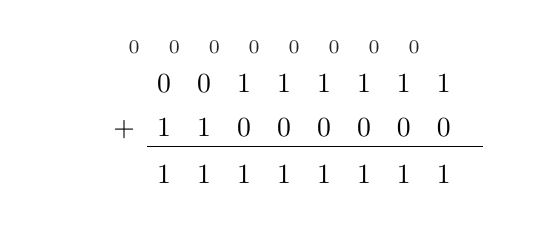
\begin{tikzpicture}[
    row 1/.style={font=\textsl,font=\scriptsize,black!85, anchor=west,
        inner sep=1.5pt},
    every node/.style={column sep=.5mm,row sep=1mm}]
    \matrix (m) [matrix of math nodes,
        nodes in empty cells,
        %nodes=draw
    ] 
    {
        &  &  & 0 & 0 & 0  & 0 & 0 & 0 & 0 & 0 &    &  &                   \\
        &  &  &   & 0 & 0  & 1 & 1 & 1 & 1 & 1 & 1  &  &[10mm]      \\
        &  &  & + & 1 & 1  & 0 & 0 & 0 & 0 & 0 & 0  &  &            \\ 
        &  &  &   & 1 & 1  & 1 & 1 & 1 & 1 & 1 & 1  &  &            \\                                                  
    };

    \draw[-,color=black,semithick] (m-3-5.south west) -- (m-3-13.south east);

\end{tikzpicture}
\end{center}

\item 136\textsubscript{10}+192\textsubscript{10}=10001000\textsubscript{2}+11000000\textsubscript{2}=11001000\textsubscript{2} $\Rightarrow$ ultimo riporto uguale a 1 $\Rightarrow$ overflow


\begin{center}
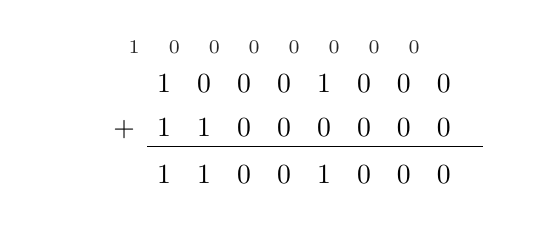
\begin{tikzpicture}[
    row 1/.style={font=\textsl,font=\scriptsize,black!85, anchor=west,
        inner sep=1.5pt},
    every node/.style={column sep=.5mm,row sep=1mm}]
    \matrix (m) [matrix of math nodes,
        nodes in empty cells,
        %nodes=draw
    ] 
    {
        &  &  & 1 & 0 & 0  & 0 & 0 & 0 & 0 & 0 &    &  &                   \\
        &  &  &   & 1 & 0  & 0 & 0 & 1 & 0 & 0 & 0  &  &[10mm]      \\
        &  &  & + & 1 & 1  & 0 & 0 & 0 & 0 & 0 & 0  &  &            \\ 
        &  &  &   & 1 & 1  & 0 & 0 & 1 & 0 & 0 & 0  &  &            \\                                                  
    };

    \draw[-,color=black,semithick] (m-3-5.south west) -- (m-3-13.south east);

\end{tikzpicture}
\end{center}

\item 136\textsubscript{10}+35\textsubscript{10}=10001000\textsubscript{2}+00100011\textsubscript{2}=10101011\textsubscript{2} $\Rightarrow$ ultimo riporto uguale a 0 $\Rightarrow$ no overflow

\begin{center}
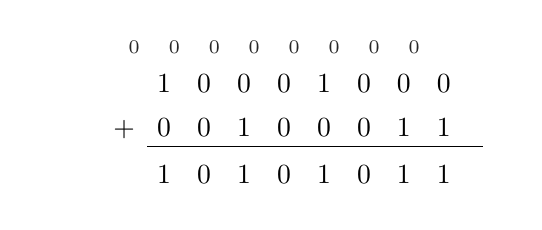
\begin{tikzpicture}[
    row 1/.style={font=\textsl,font=\scriptsize,black!85, anchor=west,
        inner sep=1.5pt},
    every node/.style={column sep=.5mm,row sep=1mm}]
    \matrix (m) [matrix of math nodes,
        nodes in empty cells,
        %nodes=draw
    ] 
    {
        &  &  & 0 & 0 & 0  & 0 & 0 & 0 & 0 & 0 &    &  &                   \\
        &  &  &   & 1 & 0  & 0 & 0 & 1 & 0 & 0 & 0  &  &[10mm]      \\
        &  &  & + & 0 & 0  & 1 & 0 & 0 & 0 & 1 & 1  &  &            \\ 
        &  &  &   & 1 & 0  & 1 & 0 & 1 & 0 & 1 & 1  &  &            \\                                                  
    };

    \draw[-,color=black,semithick] (m-3-5.south west) -- (m-3-13.south east);

\end{tikzpicture}
\end{center}

\item 63\textsubscript{10}+44\textsubscript{10}=00111111\textsubscript{2}+00101100\textsubscript{2}=01101011\textsubscript{2} $\Rightarrow$ ultimo riporto uguale a 1 $\Rightarrow$ no overflow

\begin{center}
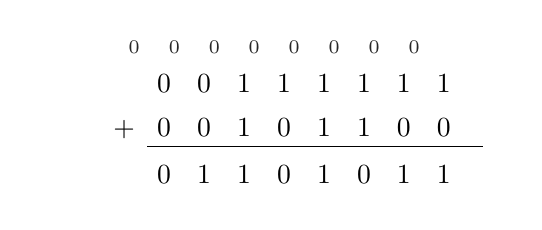
\begin{tikzpicture}[
    row 1/.style={font=\textsl,font=\scriptsize,black!85, anchor=west,
        inner sep=1.5pt},
    every node/.style={column sep=.5mm,row sep=1mm}]
    \matrix (m) [matrix of math nodes,
        nodes in empty cells,
        %nodes=draw
    ] 
    {
        &  &  & 0 & 0 & 0  & 0 & 0 & 0 & 0 & 0 &    &  &                   \\
        &  &  &   & 0 & 0 & 1 & 1 & 1 & 1 & 1 & 1  &  &[10mm]      \\
        &  &  & + & 0 & 0 & 1 & 0 & 1 & 1 & 0 & 0  &  &            \\ 
        &  &  &   & 0 & 1 & 1 & 0 & 1 & 0 & 1 & 1  &  &            \\                                                  
    };

    \draw[-,color=black,semithick] (m-3-5.south west) -- (m-3-13.south east);

\end{tikzpicture}
\end{center}

\end{enumerate}

\section{Somma e sottrazione tra numeri binari con segno}


Considerando le operazioni tra numeri binari con segno le cose si complicano leggermente, ad esempio per eseguire sottrazioni del tipo $A-B$ conviene riscrivere l'operazione come una addizione nel seguente modo:

$$ A+(-B) $$

\noindent Dobbiamo solo capire come esprimere $-B$ in binario.\\

\noindent La notazione scelta per la rappresentazione dei numeri con segno  \`e quella basata sul \textbf{complemento a due}.
Dato un numero positivo $n$ (con bit di segno uguale a 0), per ricavare il corrispettivo negativo $-n$ possiamo utilizzare uno dei due algoritmi di cambio segno:
\begin{itemize}
\item Complemento a 1 del numero $n$ e somma 1
\item Complemento a 1 di tutti i bit a sinistra della cifra 1 meno significativa
\end{itemize}

\noindent Per calcolare il valore corrispondente in decimale usiamo la seguente formula:

$$
-1\cdot 2^{n-1}+d_{n-2}\cdot 2^{n-2}+\dots+ d_{1}\cdot 2^{1}+d_{0}\cdot 2^{0}
$$

Infine ricordiamo che anche nel caso di operazioni tra numeri con segno esiste la possibilit\`a di generare overflow. La tabella riassuntiva \`e la seguente:

\begin{figure}
  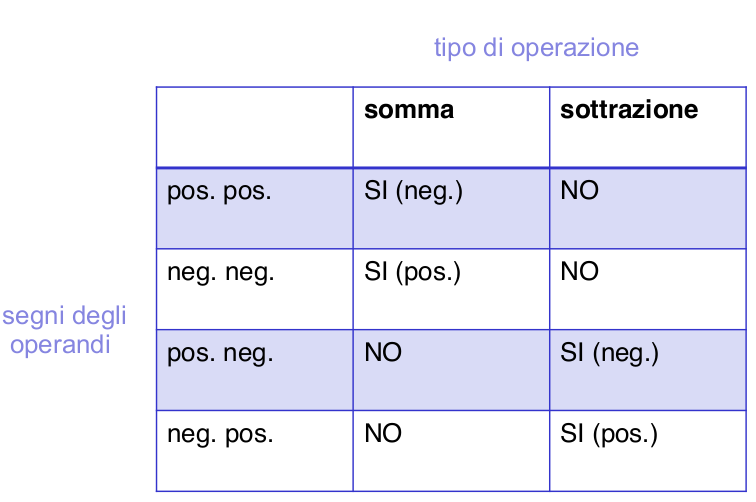
\includegraphics[width=0.7\linewidth]{overflow.png}
  \caption{Tabella riassuntiva overflow.}
\end{figure}

\subsubsection*{Esercizi}
Tradurre in complemento a due su 8 bit i numeri decimali che seguono ed eseguire le operazioni indicate sempre su 8 bit. Verificare se vi \`e overflow motivando la risposta:

\begin{enumerate}
    \item $110_{10}+120_{10}$
    \item $110_{10}-120_{10}$
    \item $-35_{10}-44_{10}$
    \item $-127_{10}-8_{10}$
\end{enumerate}

\subsubsection*{Soluzioni}

\begin{enumerate}
    \item Convertiamo i numeri da decimale a binario $+110_{10}=01101110_{2}$ mentre $+120_{10}=01111000_{2}$. Osserviamo che entrambi i numeri sono rappresentabili in complemento a due su 8 bit. Proseguiamo eseguendo la somma:

\begin{center}
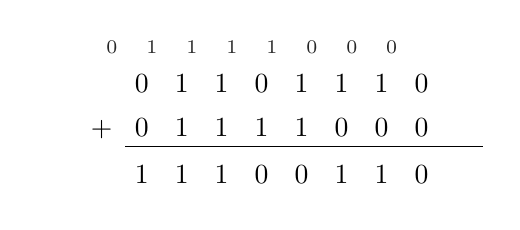
\begin{tikzpicture}[
    row 1/.style={font=\textsl,font=\scriptsize,black!85, anchor=west,
        inner sep=1.5pt},
    every node/.style={column sep=.5mm,row sep=1mm}]
    \matrix (m) [matrix of math nodes,
        nodes in empty cells,
        %nodes=draw
    ] 
    {
        &  & 0& 1 & 1 & 1 & 1 & 0 & 0 & 0 &    &  &                   \\
        &  &  & 0 & 1 & 1 & 0 & 1 & 1 & 1 & 0  &  &[10mm]      \\
        &  & +& 0 & 1 & 1 & 1 & 1 & 0 & 0 & 0  &  &            \\ 
        &  &  & 1 & 1 & 1 & 0 & 0 & 1 & 1 & 0  &  &            \\                                                  
    };

    \draw[-,color=black,semithick] (m-3-4.south west) -- (m-3-13.south east);

\end{tikzpicture}
\end{center}


Il segno dei due addendi \`e concorde (somma di due positivi), ma otteniamo un numero negativo, di conseguenza vi \`e overflow. Infatti $120_{10}+110_{10} = 230_{10}$ che non \`e esprimibile su 8 bit in complemento a due. Ricordiamo che il numero massimo positivo esprimibile in complemento a due su 8 bit corrisponde a $2^{7}-1 = 127_{10}$. In alternativa possiamo applicare la regola dei riporti (ultimi due pi\`u significativi), che in questo caso sono discordi, ossia vi \`e overflow.


\item Convertiamo i numeri da decimale a binario $+110_{10}=01101110_{2}$ mentre $+120_{10}=01111000_{2}$. Osserviamo che entrambi i numeri sono rappresentabili in complemento a due su 8 bit. Riscriviamo l'operazione in:

$$110_{10} + (-120_{10}) $$

Ricaviamo l'espressione binaria in complemento a due di $-120_{10}$ l'algoritmo di cambio di segno:

$$01111000_{2} \rightarrow 10001000_{2} $$

Eseguiamo la somma:

\begin{center}
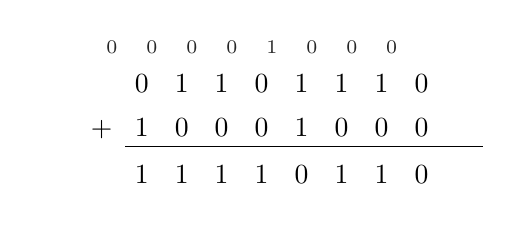
\begin{tikzpicture}[
    row 1/.style={font=\textsl,font=\scriptsize,black!85, anchor=west,
        inner sep=1.5pt},
    every node/.style={column sep=.5mm,row sep=1mm}]
    \matrix (m) [matrix of math nodes,
        nodes in empty cells,
        %nodes=draw
    ] 
    {
        &  & 0& 0 & 0 & 0 & 1 & 0 & 0 & 0 &    &  &                   \\
        &  &  & 0 & 1 & 1 & 0 & 1 & 1 & 1 & 0  &  &[10mm]      \\
        &  & +& 1 & 0 & 0 & 0 & 1 & 0 & 0 & 0  &  &            \\ 
        &  &  & 1 & 1 & 1 & 1 & 0 & 1 & 1 & 0  &  &            \\                                                  
    };

    \draw[-,color=black,semithick] (m-3-4.south west) -- (m-3-13.south east);

\end{tikzpicture}
\end{center}

Il segno dei due addendi \`e discorde non possiamo avere overflow. In alternativa possiamo applicare la regola dei riporti (ultimi due pi\`u significativi), che in questo caso sono concordi, ossia non vi \`e overflow. Per verificare la correttezza del risultato convertiamolo in decimale (ci aspettiamo $110_{10} -120_{10} = -10_{10}$).

$$-2^{7}+2^{6}+2^{5}+2^{4}+2^{2}+2^{1} = -128+64+32+16+4+2 = -128 +118 = -10_{10}$$

\item Convertiamo i numeri da decimale a binario $+35_{10}=00100011_{2}$ mentre $+44_{10}=00101100_{2}$. Osserviamo che entrambi i numeri sono rappresentabili in complemento a due su 8 bit. Riscriviamo la sottrazione in:

$$-35_{10}+(-44_{10})$$

Ricaviamo l'espressione binaria in complemento a due di $-35_{10}$ e di $-44_{10}$ eseguendo l'algoritmo di cambio di segno:

$$ 00100011_{2} \rightarrow 11011101_{2}$$
$$ 00101100_{2} \rightarrow 11010100_{2}$$

Eseguiamo la somma:

\begin{center}
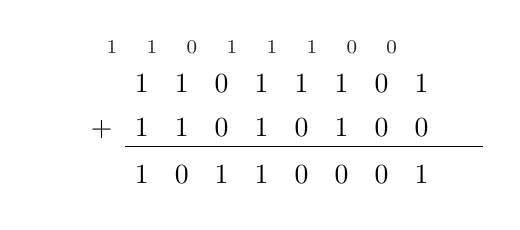
\begin{tikzpicture}[
    row 1/.style={font=\textsl,font=\scriptsize,black!85, anchor=west,
        inner sep=1.5pt},
    every node/.style={column sep=.5mm,row sep=1mm}]
    \matrix (m) [matrix of math nodes,
        nodes in empty cells,
        %nodes=draw
    ] 
    {
        &  & 1& 1 & 0 & 1 & 1 & 1 & 0 & 0 &    &  &                   \\
        &  &  & 1 & 1 & 0 & 1 & 1 & 1 & 0 & 1  &  &[10mm]      \\
        &  & +& 1 & 1 & 0 & 1 & 0 & 1 & 0 & 0  &  &            \\ 
        &  &  & 1 & 0 & 1 & 1 & 0 & 0 & 0 & 1  &  &            \\                                                  
    };

    \draw[-,color=black,semithick] (m-3-4.south west) -- (m-3-13.south east);

\end{tikzpicture}
\end{center}

Il segno dei due addendi \`e concorde (somma di due negativi) ed anche il risultato della somma \`e negativo, di conseguenza  non vi \`e overflow. In alternativa possiamo applicare la regola dei riporti (ultimi due pi\`u significativi), che in questo caso sono concordi, ossia non vi \`e overflow. Per verificare l'esattezza del risultato convertiamolo in decimale (ci aspettiamo $-35_{10}-44_{10} = -79_{10}$)

$$-2^{7}+2^{5}+2^{4}+2^{0} = -128+32+16+1 = -128 + 49 = -79_{10}$$


\item Convertiamo i numeri da decimale a binario $+127_{10}=01111111_{2}$ mentre $+8_{10}=00001000_{2}$. Osserviamo che entrambi i numeri sono rappresentabili in complemento a due su 8 bit. Riscriviamo la sottrazione in:

$$-127_{10}+(-8_{10})$$

Ricaviamo l'espressione binaria in complemento a due di $-127_{10}$ e di $-8_{10}$ eseguendo l'algoritmo di cambio di segno:

$$ 01111111_{2} \rightarrow 10000001_{2}$$
$$ 00001000_{2} \rightarrow 11111000_{2}$$

Eseguiamo la somma:

\begin{center}
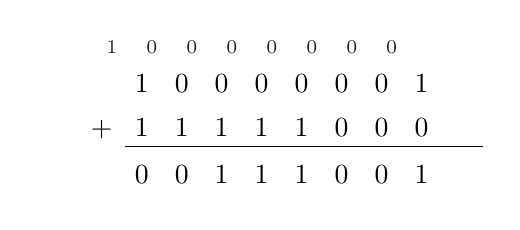
\begin{tikzpicture}[
    row 1/.style={font=\textsl,font=\scriptsize,black!85, anchor=west,
        inner sep=1.5pt},
    every node/.style={column sep=.5mm,row sep=1mm}]
    \matrix (m) [matrix of math nodes,
        nodes in empty cells,
        %nodes=draw
    ] 
    {
        &  & 1& 0 & 0 & 0 & 0 & 0 & 0 & 0 &    &  &                   \\
        &  &  & 1 & 0 & 0 & 0 & 0 & 0 & 0 & 1  &  &[10mm]      \\
        &  & +& 1 & 1 & 1 & 1 & 1 & 0 & 0 & 0  &  &            \\ 
        &  &  & 0 & 0 & 1 & 1 & 1 & 0 & 0 & 1  &  &            \\                                                  
    };

    \draw[-,color=black,semithick] (m-3-4.south west) -- (m-3-13.south east);

\end{tikzpicture}
\end{center}

Il segno dei due addendi \`e concorde (somma di due negativi), ma il risultato della somma \`e positivo, di conseguenza  vi \`e overflow. Infatti $-127_{10}-8_{10} =-135_{10}$ che non \`e esprimibile su 8 bit in complemento a due. Ricordiamo che il numero massimo negativo rappresentabile in complemento a due con 8 bit corrisponde a $-2^7 = -128_{10}$. In alternativa possiamo applicare la regola dei riporti (ultimi due pi\`u significativi), che in questo caso sono discordi, ossia vi \`e overflow.

\end{enumerate}

\end{document}